\documentclass[11pt]{article}

% ---------------------------------------------------------------------------
% Communication-Aware ML for MDD — full project report
% ---------------------------------------------------------------------------
\usepackage[utf8]{inputenc}
\usepackage[T1]{fontenc}
\usepackage{lmodern}
\usepackage[margin=1in]{geometry}
\usepackage{amsmath,amssymb}
\usepackage{graphicx}
\usepackage{booktabs}
\usepackage{caption}
\usepackage{subcaption}
\usepackage[table]{xcolor}
\usepackage{microtype}
\usepackage{array}
\usepackage{tikz}
\usetikzlibrary{shapes.geometric,arrows.meta,positioning,fit,backgrounds,calc}
\usepackage[colorlinks=true,linkcolor=blue!55!black,citecolor=blue!55!black,
            urlcolor=blue!55!black]{hyperref}

\definecolor{phaseA}{HTML}{2C6E8F}
\definecolor{phaseB}{HTML}{8A4FAF}
\definecolor{phaseC}{HTML}{C0392B}
\definecolor{phaseD}{HTML}{1E8449}
\definecolor{lightgray}{HTML}{F2F2F2}

\newcommand{\factorfour}{\textbf{Factor~4}}
\newcommand{\code}[1]{\texttt{\small #1}}

\captionsetup{font=small,labelfont=bf}

\title{\textbf{Communication-Aware Machine Learning for Major Depressive
Disorder}\\[4pt]
\large Testing a microglia\,$\rightarrow$\,neuron communication axis from
single-nucleus RNA-seq of the human prefrontal cortex}

\author{Giorgos Boulogeorgos, Andreas Mici \\[4pt]
\small National and Kapodistrian University of Athens (NKUA) \\
\small MSc in Data Science and Information Technologies \\[3pt]
\small MLCB Team Project --- Supervisor: Prof.\ E.~Manolakos \\[2pt]
\small Re-analysis of Maitra \textit{et al.}
(2023), \textit{Nature Communications} \textbf{14}, 2912}
\date{June 2026}

\begin{document}
\maketitle

\begin{abstract}
\noindent
Maitra \textit{et al.} (2023) reported that, in major depressive disorder
(MDD), the strongest single-nucleus transcriptomic signal is carried by
\emph{microglia} (cluster \code{Mic1}) in females and by a \emph{deep-layer
excitatory neuron} (cluster \code{ExN10\_L46}) in males, and presented these as
two separate, sex-specific findings. We test the hypothesis that they are the
two ends of a single \emph{microglia\,$\rightarrow$\,neuron communication axis}
whose apparent sex-specificity is partly an artefact of per-cluster
differential-expression analysis treating cell types as isolated. Re-analysing
their 71-donor dlPFC dataset ($\sim$160k nuclei; GSE213982\,+\,GSE144136), we
(A)~reproduce the cell-type signal, (B)~infer \emph{per-donor} ligand--receptor
networks with LIANA and compress them into five communication programs by
non-negative tensor (CP/PARAFAC) decomposition, and (C)~train donor-level
case/control classifiers on three feature sets---expression-only,
communication-only, and combined---under rigorous, leakage-controlled repeated
nested cross-validation, with SHAP for interpretation. A single data-driven
program (\factorfour, an \mbox{endothelial\,+\,microglia\,$\rightarrow$\,}\code{ExN10\_L46}
axis) emerges as the dominant, cohort-clean, MDD-leaning communication signal;
it is higher in MDD donors of \emph{both} sexes (stronger in males, standalone
AUC~0.702, $p=0.05$) and becomes the \#1 communication factor by SHAP once
factors are re-estimated inside each fold. However, when these factors compete
directly with microglial/neuronal gene expression, feature selection keeps only
genes and discards every factor: the axis carries \emph{no predictive
information independent of microglial transcriptional state} at $n=71$. The
biology of the hypothesis is directionally supported; the communication
representation does not add value over expression for donor-level
classification.
\end{abstract}

\medskip
\noindent\textbf{Keywords:} major depressive disorder; single-nucleus RNA-seq;
cell--cell communication; ligand--receptor inference; tensor decomposition;
interpretable machine learning; microglia; prefrontal cortex.
\bigskip

% ===========================================================================
\section{Introduction}
% ===========================================================================

Major depressive disorder (MDD) is a leading cause of disability whose
molecular substrate in the human brain remains poorly resolved. Single-nucleus
RNA sequencing (snRNA-seq) of the dorsolateral prefrontal cortex (dlPFC) has
made it possible to ask which \emph{cell types} carry the disease signal.
Maitra \textit{et al.}~\cite{maitra2023} profiled $\sim$160{,}000 nuclei from
71 donors and found that the strongest case/control differences localise to
\textbf{microglia} (fine cluster \code{Mic1}) in \emph{female} donors and to a
\textbf{deep-layer excitatory neuron} population (fine cluster
\code{ExN10\_L46}) in \emph{male} donors. These were reported as two distinct,
sex-specific results.

\paragraph{Hypothesis.} We hypothesise that the female microglial signal and
the male excitatory-neuron signal are not independent but are \emph{two ends of
one microglia\,$\rightarrow$\,neuron communication axis}---microglia as sender,
deep-layer neuron as receiver. Under this view, the apparent sex-specificity is
partly an artefact of per-cluster differential-expression (DEG) analysis, which
treats each cell type in isolation and therefore cannot see a signal that lives
\emph{between} cell types. If the hypothesis holds, explicitly modelling
cell--cell communication should expose a shared axis that is active in MDD
donors of both sexes. This report develops that test end-to-end and reports an
honest, leakage-controlled answer.

\paragraph{Scope.} The project was deliberately narrowed from the original
proposal: no scVI integration benchmark and no graph neural network ($n=71$
donors is far too few to train one). The core deliverable is the
interpretable machine-learning comparison of expression vs.\ communication
features at the donor level.

% ===========================================================================
\section{Materials and Methods}
% ===========================================================================

\subsection{Data}

We re-use the combined count matrix released by Maitra \textit{et al.}, which
merges the female cohort (GSE213982) and the male cohort (GSE144136) into a
single dlPFC (Brodmann area~9) snRNA-seq matrix. Key facts, verified during
Phase~A (Table~\ref{tab:data}):

\begin{table}[h]
\centering
\caption{Dataset summary (after the authors' quality control).}
\label{tab:data}
\small
\begin{tabular}{lr}
\toprule
Property & Value \\
\midrule
Donors (CV unit) & \textbf{71} \\
\quad MDD (death by suicide) / Control & 37 / 34 \\
\quad Female / Male & 38 / 33 \\
\quad Female MDD / Control & 20 / 18 \\
\quad Male MDD / Control & 17 / 16 \\
Nuclei (high-quality) & 160{,}711 \\
Genes & 36{,}588 \\
Region / assay & dlPFC (BA9), 10x snRNA-seq \\
\bottomrule
\end{tabular}
\end{table}

Two dataset properties simplified the pipeline. First, the GEO file
\code{GSE213982\_\allowbreak combined\_\allowbreak counts\_\allowbreak
matrix.mtx.gz} \emph{already contains both sexes}---the authors merged the male cohort into it---so only the male SOFT
metadata is needed for diagnosis labels. Second, the authors' cell-type
annotations are baked into each cell identifier
(\code{donor.barcode.broad.fine}, e.g.\ \code{F1.AAAC\ldots-1.Mic.Mic1}),
giving both 7 broad classes and 41 fine clusters for free. One subtlety was
handled explicitly: donor \code{M24} appears twice (\code{M24}\,+\,\code{M24\_2},
two sequencing runs of one individual) and is merged to a single donor,
otherwise its two halves could split across CV folds and leak donor identity
(72~donor tokens~$\rightarrow$~71~donors).

\paragraph{Confound to track throughout.} Sex is perfectly confounded with
cohort/library (females $=$~GSE213982, males $=$~GSE144136). Any
train-on-one-sex/test-on-the-other split is therefore also a train/test
across-batch split, so a failure to generalise could be batch rather than
biology. This single fact reshaped the evaluation design (Section~\ref{sec:phaseC}).

% ===========================================================================
\subsection{Pipeline overview}
% ===========================================================================

The analysis proceeds in three phases (Figure~\ref{fig:pipeline})---reproduction
(A), cell--cell communication inference (B) and machine learning (C)---followed
by an interpretability and hypothesis-testing layer (Phase~D, referred to as
Step~4 in the code). Each expensive step is checkpointed so a runtime timeout
never costs more than one step.

\begin{figure}[h]
\centering
\resizebox{\textwidth}{!}{%
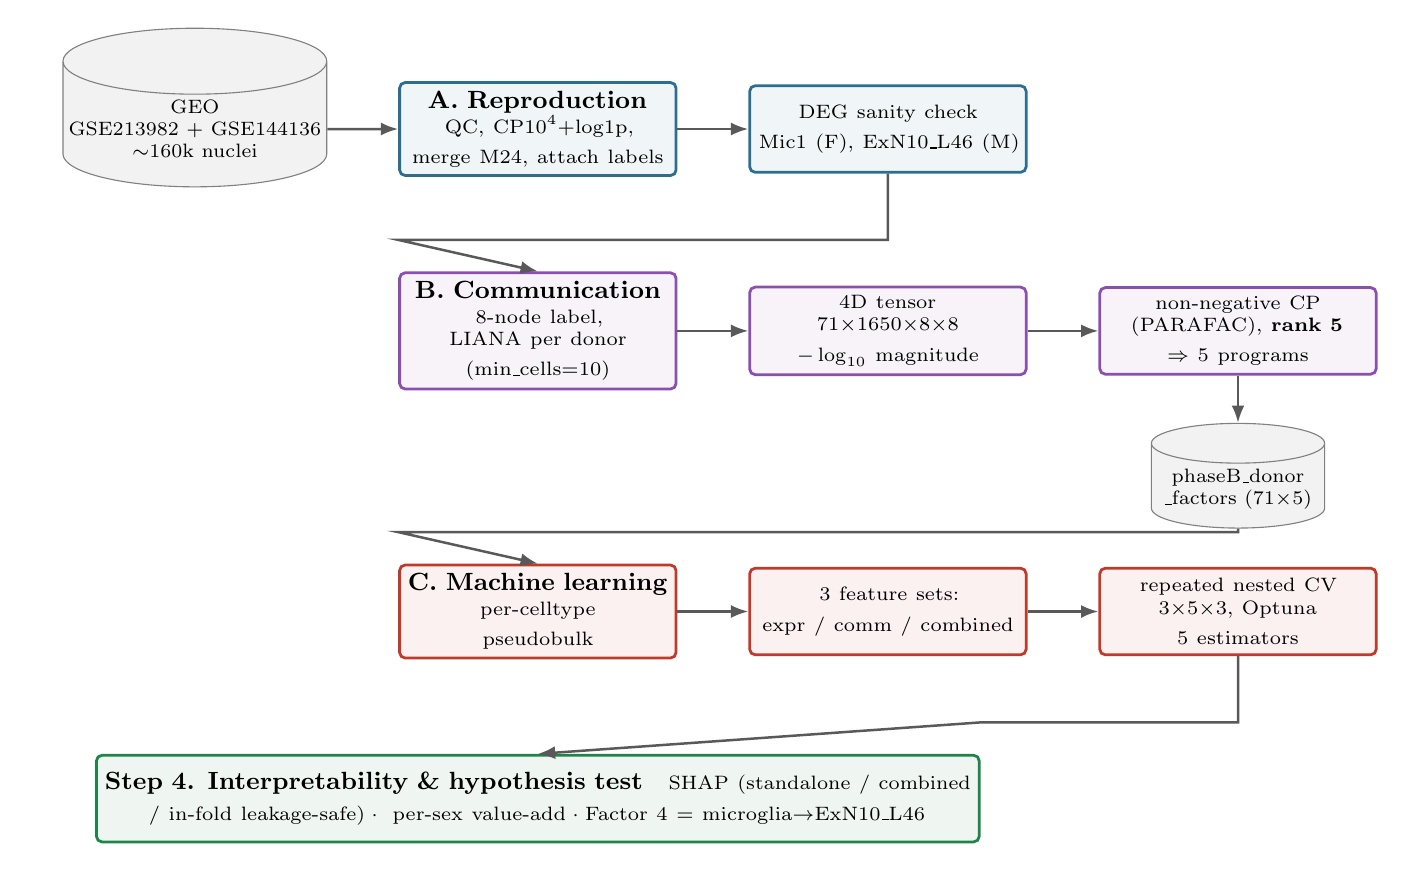
\begin{tikzpicture}[
  node distance=6mm and 9mm,
  font=\small,
  box/.style={rectangle, rounded corners=2pt, draw=#1, line width=1pt,
              fill=#1!7, text width=33mm, minimum height=11mm, align=center,
              inner sep=3pt},
  data/.style={cylinder, shape border rotate=90, aspect=0.25, draw=gray,
               fill=lightgray, minimum width=22mm, minimum height=10mm,
               align=center, inner sep=2pt, font=\scriptsize},
  arr/.style={-{Latex[length=2.2mm]}, line width=0.9pt, gray!70!black},
  lab/.style={font=\bfseries\footnotesize}
]

% ---- raw data ----
\node[data] (geo) {GEO\\GSE213982 + GSE144136\\$\sim$160k nuclei};

% ---- Phase A ----
\node[box=phaseA, right=of geo] (a1)
  {\textbf{A. Reproduction}\\[1pt]\scriptsize QC, CP10$^4$+log1p,\\merge M24,
   attach labels};
\node[box=phaseA, right=of a1] (a2)
  {\scriptsize DEG sanity check\\Mic1 (F), ExN10\_L46 (M)};

% ---- Phase B ----
\node[box=phaseB, below=12mm of a1] (b1)
  {\textbf{B. Communication}\\[1pt]\scriptsize 8-node label,\\LIANA per donor\\(min\_cells=10)};
\node[box=phaseB, right=of b1] (b2)
  {\scriptsize 4D tensor\\$71{\times}1650{\times}8{\times}8$\\$-\log_{10}$ magnitude};
\node[box=phaseB, right=of b2] (b3)
  {\scriptsize non-negative CP\\(PARAFAC), \textbf{rank 5}\\$\Rightarrow$ 5 programs};

% ---- Phase C ----
\node[box=phaseC, below=22mm of b1] (c1)
  {\textbf{C. Machine learning}\\[1pt]\scriptsize per-celltype\\pseudobulk};
\node[box=phaseC, right=of c1] (c2)
  {\scriptsize 3 feature sets:\\expr / comm / combined};
\node[box=phaseC, right=of c2] (c3)
  {\scriptsize repeated nested CV\\$3{\times}5{\times}3$, Optuna\\5 estimators};

% ---- Step 4 ----
\node[box=phaseD, below=12mm of c1, text width=110mm] (d1)
  {\textbf{Step 4. Interpretability \& hypothesis test}\quad\scriptsize
   SHAP (standalone / combined / in-fold leakage-safe)\;$\cdot$\;
   per-sex value-add\;$\cdot$\;Factor 4 = microglia$\rightarrow$ExN10\_L46};

% ---- data artefacts under B ----
\node[data, below=6mm of b3] (bf)
  {phaseB\_donor\\\_factors (71$\times$5)};

% arrows
\draw[arr] (geo) -- (a1);
\draw[arr] (a1) -- (a2);
\draw[arr] (a2.south) |- ($(b1.north west)+(0,4mm)$) -- (b1.north);
\draw[arr] (b1) -- (b2);
\draw[arr] (b2) -- (b3);
\draw[arr] (b3) -- (bf);
\draw[arr] (bf.south) |- ($(c1.north west)+(0,4mm)$) -- (c1.north);
\draw[arr] (c1) -- (c2);
\draw[arr] (c2) -- (c3);
\draw[arr] (c3.south) |- ($(d1.north east)+(0,4mm)$) -- (d1.north);

% phase rails (labels on the left)
\node[lab, phaseA, left=2mm of geo, rotate=90, anchor=south] {};
\end{tikzpicture}%
}
\caption{End-to-end pipeline. \textbf{Phase A} loads, normalises and annotates
the combined matrix and confirms the cell-type signal. \textbf{Phase B} infers
ligand--receptor scores \emph{per donor} (LIANA), arranges them as a 4D tensor
(donor\,$\times$\,L--R pair\,$\times$\,sender\,$\times$\,receiver) and
compresses it into five communication \emph{programs} by non-negative CP
decomposition. \textbf{Phase C} builds per-donor pseudobulk expression and
compares three feature sets under repeated nested cross-validation.
\textbf{Step~4} interprets the models with SHAP and runs the directed
hypothesis test on the microglia\,$\rightarrow$\,\code{ExN10\_L46} program.}
\label{fig:pipeline}
\end{figure}

% ===========================================================================
\subsection{Phase A --- Reproduction}
% ===========================================================================

Because the authors already performed QC \emph{and} annotation, Phase~A is
leaner than a full reproduction: we do not re-cluster (which would be stochastic
and the authors' annotations are validated). Phase~A (i)~streams the $\sim$1.1\,GB
matrix into an \code{AnnData} object, parses the cell string into
donor/barcode/broad/fine, merges \code{M24\_2}$\rightarrow$\code{M24}, and
attaches sex and diagnosis; (ii)~normalises \code{.X} to counts-per-$10^4$ then
\code{log1p} (Scanpy~\cite{scanpy}), preserving raw counts in
\code{.layers['counts']} (pseudobulk in
Phase~C needs raw); and (iii)~runs a nucleus-level Wilcoxon DEG sanity check
(MDD vs.\ Control, within sex) on \code{Mic1} and \code{ExN10\_L46}. Both show
strong signal---\code{Mic1} (female) synaptic/adhesion genes up, \code{ExN10\_L46}
(male) metabolic/synaptic genes (\code{GAPDH}, \code{PKM}, \code{CKB},
\code{VAMP2}, \code{SNCB}) down.

\paragraph{Honest caveat.} Nucleus-level Wilcoxon pseudoreplicates (nuclei from
one donor are not independent), inflating the count of ``significant'' DEGs. We
confirmed the \code{ExN10\_L46} signal holds at the donor level (median
per-donor expression); definitive donor-level statistics come later via
pseudobulk---which is exactly why the authors used pseudobulk rather than
nucleus-level tests. The Phase~A checkpoint
(\code{phaseA\_final\_for\_cellchat.h5ad}) carries normalised \code{.X}, raw
\code{.layers['counts']}, and \code{.obs} columns
\code{donor\_id, cell\_type\_broad, cell\_type\_fine, sex, condition, dataset}.

% ===========================================================================
\subsection{Phase B --- Cell--cell communication}
% ===========================================================================

\paragraph{Three deliberate methodology changes} (agreed before building) moved
Phase~B away from the original CellChat plan:

\begin{enumerate}
\item \textbf{LIANA (Python), not CellChat (R).} LIANA's
\code{rank\_aggregate.by\_sample}~\cite{liana2022} performs \emph{per-donor}
ligand--receptor inference natively, avoiding fragile \code{rpy2}/R setup.
\item \textbf{Per-donor, not per-condition inference.} Running four
condition-level networks (sex\,$\times$\,diagnosis) and projecting onto donors is
\emph{degenerate}: every donor in a group receives an identical communication
vector that merely re-encodes (sex, diagnosis), so a classifier would ``work''
while learning nothing. Per-donor inference gives each of the 71 donors its own
L--R scores with real donor-to-donor variation.
\item \textbf{No leave-one-sex-out as the test} (the sex\,$=$\,cohort confound,
Section~\ref{sec:phaseC}).
\end{enumerate}

\paragraph{Granularity (hybrid, 8 nodes).} A per-donor cell-count diagnostic
showed that \code{Mic}\,$\equiv$\,\code{Mic1} in this annotation (microglia have
a single fine cluster), so there is nothing to split on the sender side. But
\code{ExN10\_L46} is only $\sim$3.4\% of \code{ExN}, so a broad
\code{Mic}$\rightarrow$\code{ExN} edge would be $\sim$96.6\% off-target. We
therefore split \emph{only} \code{ExN10\_L46} out of \code{ExN}
(remainder~$=$~\code{ExN\_other}) and keep everything else broad. Final nodes:
\code{Ast, End, ExN10\_L46, ExN\_other, InN, Mic, OPC, Oli} (\code{Mix}
dropped, leaving 156{,}911 of the 160{,}711 nuclei). With \code{min\_cells=10} per donor,
focal-edge missingness is balanced across diagnosis (Mann--Whitney $p=0.19$), so
it does not leak the label; donors below threshold in a cell type are
\emph{masked} (not imputed).

\paragraph{Tensor decomposition.} The per-donor L--R table is arranged as a 4D
tensor (\textbf{71 donors $\times$ 1650 L--R pairs $\times$ 8 senders $\times$ 8
receivers}); masked donor/cell-type slices are left as \code{NaN} so the
decomposition \emph{borrows strength across donors} rather than imputing.
Following LIANA's \code{to\_tensor\_c2c} convention, the \code{magnitude\_rank}
score (a rank in $(0,1]$ where small\,$=$\,strong) is transformed by
$-\log_{10}(x+\varepsilon)$, which both flips orientation (large\,$=$\,strong)
and reshapes it; an early bug that omitted this transform left the in-fold
factors inverted and collapsed two linear models to chance, and was fixed once
diagnosed. A non-negative CP (PARAFAC) decomposition~\cite{tensorc2c,tensorly}
with \textbf{rank~5} (justified below) yields
five \emph{communication programs}; a
donor's \emph{loading} on a program measures how active it is in that donor.
Each factor's sender, receiver and L--R loadings give its biological
interpretation.

\paragraph{Why rank~5.} Figure~\ref{fig:elbow} plots the reconstruction error as
the rank grows. As is typical for CP decompositions of noisy single-cell
communication tensors, the error declines \emph{smoothly}, with diminishing
returns rather than a sharp elbow: the first five components capture about
two-thirds of the total error reduction available over ranks~1--8
($0.66\!\rightarrow\!0.58$ by rank~5 vs.\ a further $0.58\!\rightarrow\!0.54$
across ranks~6--8), and each component past five lowers the error by
progressively less while adding another program to interpret. We therefore do
not over-read a kink that is not there; rank~5 is a deliberate \emph{parsimony /
interpretability} choice---small enough that each program admits a clear
sender\,$\rightarrow$\,receiver reading, yet large enough to resolve the dominant
batch/cohort structure (Factors~2/3/5) from the diagnosis-leaning biology
(\factorfour), matching the low single-digit ranks used in Tensor-cell2cell
workflows. The choice is validated \emph{post hoc}: the five programs cleanly
separate batch from biology (Table~\ref{tab:factors}), and the in-fold refit
re-estimates a rank-5 decomposition inside every training fold yet recovers the
same \factorfour\ ($|r|\approx0.95$; median $0.97$ across the five factors vs.\
the frozen all-donor factors).

\begin{figure}[h]
\centering
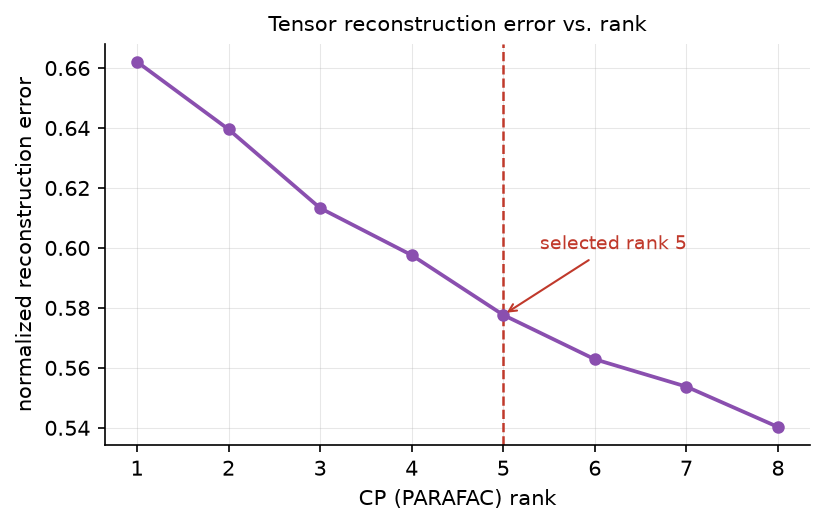
\includegraphics[width=0.62\textwidth]{figures/phaseB_reconstruction_error.png}
\caption{Tensor reconstruction error vs.\ CP (PARAFAC) rank. Normalised
Frobenius reconstruction error over the observed (unmasked) entries of the
$71\times1650\times8\times8$ communication tensor, for non-negative
decompositions of rank $1$--$8$ (single seed, \code{random\_state=0}, matching
the in-fold projector). The error decreases \emph{smoothly} with diminishing
returns rather than at a sharp elbow; rank~5 (dashed line) captures roughly
two-thirds of the reduction available across this range and was fixed for
parsimony and interpretability (see text).}
\label{fig:elbow}
\end{figure}

\begin{table}[h]
\centering
\caption{The five communication programs and their association with diagnosis
vs.\ sex/cohort (per-factor Mann--Whitney $p$). The batch confound
self-segregates into Factors 2/3/5 (strongly sex-linked, diagnosis-null) and
does \emph{not} smear into the biology. \factorfour\ is the only
diagnosis-leaning, cohort-clean program, and it is the one selected
\emph{a priori} as the microglia\,$\rightarrow$\,\code{ExN10\_L46} axis.}
\label{tab:factors}
\small
\begin{tabular}{clccl}
\toprule
Factor & Program (dominant sender\,$\rightarrow$\,receiver) & $p$(diagnosis) &
$p$(sex/cohort) & note \\
\midrule
1 & ExN\,$\rightarrow$\,ExN & 0.348 & 0.778 & no signal \\
2 & ExN\,$\rightarrow$\,Ast/OPC & 0.398 & \textbf{0.0025} & cohort/batch \\
3 & OPC/Ast\,$\rightarrow$\,mixed & 0.479 & \textbf{0.0002} & cohort/batch \\
\rowcolor{phaseC!8}
\textbf{4} & \textbf{End\,+\,Mic\,$\rightarrow$\,ExN10\_L46} &
\textbf{0.057} & 0.108 & \textbf{hypothesis program} \\
5 & mixed\,$\rightarrow$\,End & 0.886 & \textbf{0.00002} & cohort/batch \\
\bottomrule
\end{tabular}
\end{table}

\paragraph{The hypothesis program (\factorfour).} \factorfour's senders load on
\textbf{Endothelial (0.79)} and \textbf{Microglia (0.40)}; its receivers load on
\textbf{\code{ExN10\_L46} (0.54)} and \code{ExN\_other} (0.52). Its top
ligand--receptor drivers are synaptic-adhesion / glutamatergic / Ca$^{2+}$
pairs---\code{IL1RAPL1--PTPRD}, \code{CALM1--GRM5/GRM7/KCNQ5/RYR2},
\code{NRXN3--NLGN1}, \code{APP--DCC}, \code{CALM1--CACNA1C}
(\code{CACNA1C} and \code{IL1RAPL1} are psychiatric-relevant). Quantifying the
microglia-sender\,$\times$\,\code{ExN10\_L46}-receiver product gives loading
$0.40\times0.54\approx0.22$, far above any other factor---hence \factorfour\ is
the data-driven instantiation of the axis under test.

\paragraph{Honest caveats (carried forward).} $p=0.057$ is a \emph{trend}, not
significance (univariate, one factor). \factorfour's top sender is actually
Endothelial ($0.79$) $>$ Mic ($0.40$), so strictly it is a ``non-neuronal
(vascular\,+\,immune)\,$\rightarrow$\,deep-layer neuron'' program rather than pure
microglia. Selecting \factorfour\ by \emph{biology} (not by $p$-value) keeps
this a legitimate \emph{directed} test.

% ===========================================================================
\subsection{Phase C --- Machine learning}
\label{sec:phaseC}
% ===========================================================================

\paragraph{Feature sets.} Three donor-level matrices are compared:
\begin{enumerate}
\item \textbf{Expression-only} --- per-cell-type pseudobulk (raw counts summed
per donor$\times$cell type, then logCPM); the baseline.
\item \textbf{Communication-only} --- the 5 factor loadings.
\item \textbf{Combined} --- pseudobulk + 5 factors.
\end{enumerate}

\paragraph{Communication vs.\ expression, in plain terms.}
\emph{Expression} features are raw gene-activity readouts: for each donor and
cell type, how much each gene is switched on (e.g.\ how much \code{IL1RAPL1}
microglia make). \emph{Communication} features are \emph{relational}: they score
how strongly a ligand from a \emph{sender} cell type can engage its receptor on
a \emph{receiver} cell type, then compress thousands of such sender$\rightarrow$
receiver L--R scores into 5 programs. Crucially, communication is \emph{computed
from} expression (a ligand's ``signal'' is essentially its gene expression), so
the two are not independent---which is exactly why the combined-feature
comparison below is the decisive test of whether communication adds anything.

\paragraph{Evaluation: within-sex value-add (not leave-one-sex-out).} Because
sex is perfectly confounded with cohort, we evaluate with \emph{pooled}
donor-level CV stratified by \textbf{sex\,$\times$\,diagnosis} (diagnosis is
balanced within each sex: F~20/18, M~17/16), so a fold never crosses the batch.
The hypothesis test becomes: does adding communication beat expression-only, and
is \factorfour's importance \emph{shared across sexes}?

\paragraph{Model selection and validation.} We use \emph{repeated nested
cross-validation}: 3 rounds $\times$ 5 outer folds $\times$ 3 inner folds, with
20 Optuna~\cite{optuna} trials per inner search, evaluating five
estimators---logistic regression (LR), Gaussian naive Bayes (GNB), linear
discriminant analysis (LDA) and random forest (RF) from
scikit-learn~\cite{sklearn}, plus XGBoost~\cite{xgboost}. Bootstrap 95\% confidence
intervals are reported. Feature pipelines are fit \emph{inside} the training
fold: a variance top-1000 prefilter (\code{VarianceTopK}) followed by mRMR
selection of $k=15$ features (\code{MRMRSelector}, relevance\,$=$\,mutual
information)~\cite{mrmr}.

\paragraph{Leakage rules (non-negotiable).}
\begin{itemize}
\item CV unit\,$=$\,donor, one row per donor (\code{M24} merged), stratified by
sex\,$\times$\,diagnosis.
\item All expression feature selection / variance prefilter / scaling is fit on
the training fold only.
\item \textbf{Tensor leakage removed (rigorous path).} The Phase~B rank-5
decomposition was fit on all 71 donors (unsupervised; the leak is mild). For
the headline numbers we \emph{re-fit the tensor inside each outer-train fold}
(\code{TensorFactorProjector}: non-negative PARAFAC on train donors, then NNLS
projection of held-out donors onto the fixed factors). Because non-negative CP
has no sign ambiguity (only permutation), in-fold components are matched to the
canonical Factor~1\ldots5 by $|\mathrm{corr}|$ Hungarian assignment.
\end{itemize}

% ===========================================================================
\section{Results}
% ===========================================================================

\subsection{Donor-level classification}

Table~\ref{tab:auc} reports median test AUC (with 95\% bootstrap CI) and median
MCC for each feature set $\times$ estimator under the rigorous CV.

\begin{table}[h]
\centering
\caption{Rigorous repeated-nested-CV performance (median AUC [95\% CI]; median
MCC). Communication-only carries weak but real signal in the \emph{linear}
models (LR/GNB/LDA $\approx$ 0.633) and is at chance for tree models; expression
is the stronger baseline (XGB 0.714); combined never CI-separates from
expression.}
\label{tab:auc}
\small
\setlength{\tabcolsep}{5pt}
\begin{tabular}{l ccc ccc ccc}
\toprule
& \multicolumn{3}{c}{\textbf{Communication}} &
  \multicolumn{3}{c}{\textbf{Expression}} &
  \multicolumn{3}{c}{\textbf{Combined}} \\
\cmidrule(lr){2-4}\cmidrule(lr){5-7}\cmidrule(lr){8-10}
Est. & AUC & 95\% CI & MCC & AUC & 95\% CI & MCC & AUC & 95\% CI & MCC \\
\midrule
LR  & 0.633 & [0.56,0.73] & 0.04 & 0.646 & [0.61,0.73] & 0.26 &
      \textbf{0.694} & [0.55,0.76] & \textbf{0.42} \\
GNB & 0.633 & [0.58,0.69] & 0.17 & 0.643 & [0.50,0.71] & 0.17 &
      0.673 & [0.54,0.73] & 0.22 \\
LDA & 0.633 & [0.56,0.76] & 0.05 & 0.667 & [0.57,0.71] & 0.25 &
      0.653 & [0.50,0.77] & 0.15 \\
RF  & 0.536 & [0.50,0.59] & 0.00 & 0.688 & [0.63,0.76] & 0.20 &
      0.667 & [0.57,0.71] & 0.15 \\
XGB & 0.490 & [0.40,0.61] & $-0.14$ & \textbf{0.714} & [0.61,0.73] & 0.29 &
      \textbf{0.714} & [0.63,0.83] & 0.29 \\
\bottomrule
\end{tabular}
\end{table}

\paragraph{Value-add (combined $-$ expression).} Positive on average but
\emph{not} CI-separated: LR $+0.048$~AUC ($+0.158$~MCC), GNB $+0.031$; LDA/RF
slightly negative; XGB $0.714\rightarrow0.714$. The honest read: communication
carries weak \emph{real} signal (linear models only) but adds no statistically
demonstrable value beyond expression at $n=71$. These rigorous numbers
\emph{replace} the earlier pragmatic (all-donor-factor) numbers, which were
mildly leak-inflated.

\subsection{Phase D (Step~4) --- interpretation and the directed hypothesis test}

We probe \factorfour\ from three angles with SHAP~\cite{shap} (signed log-odds
contributions; colour\,$=$\,feature value, red high / blue low).

\paragraph{(i) Standalone direction and sex.} \factorfour\ is higher in MDD
donors in \emph{both} sexes (consistent direction). Standalone it discriminates
MDD with AUC~0.632 overall, concentrated in \textbf{males} (AUC~0.702,
Mann--Whitney $p=0.05$) more than females (0.578, $p=0.42$). In the
communication-only LR (the only comm model above chance), linear-SHAP ranks
\factorfour\ \textbf{\#2 of 5}, comparably across sexes (F~0.234, M~0.227)
(Figure~\ref{fig:beeswarm-comm}).

\begin{figure}[h]
\centering
\begin{subfigure}{0.6\textwidth}
  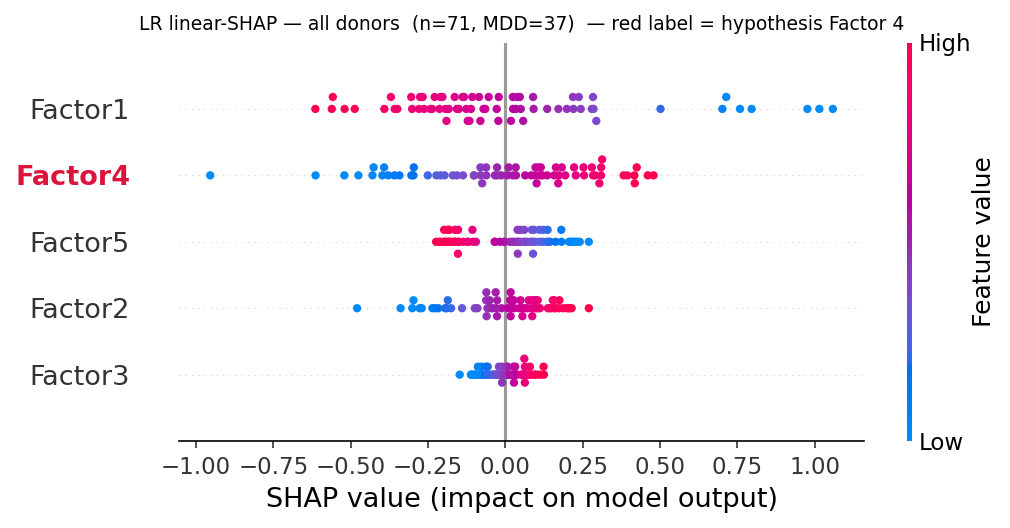
\includegraphics[width=\linewidth]{figures/step4_shap_beeswarm_overall.png}
  \caption{All donors ($n=71$).}
\end{subfigure}
\\[4pt]
\begin{subfigure}{0.49\textwidth}
  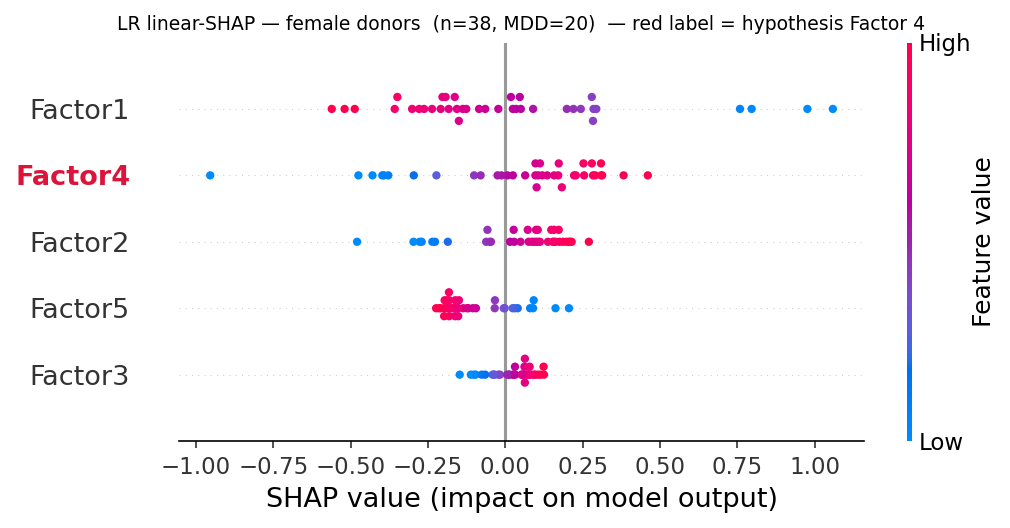
\includegraphics[width=\linewidth]{figures/step4_shap_beeswarm_female.png}
  \caption{Female donors ($n=38$).}
\end{subfigure}\hfill
\begin{subfigure}{0.49\textwidth}
  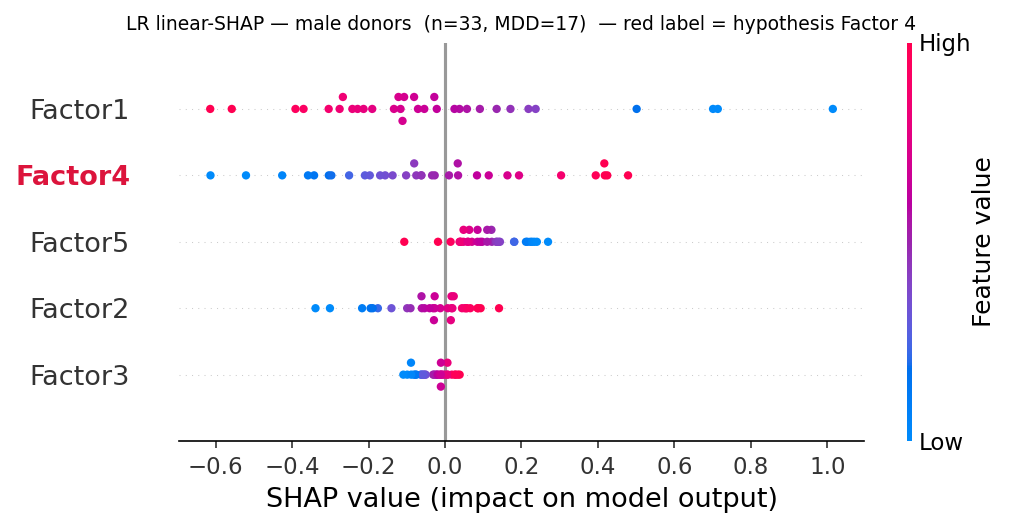
\includegraphics[width=\linewidth]{figures/step4_shap_beeswarm_male.png}
  \caption{Male donors ($n=33$).}
\end{subfigure}
\caption{Communication-only logistic-regression SHAP beeswarm (the five factor
loadings). \factorfour\ (red label) carries among the largest mean$|$SHAP$|$ and
its \emph{high} values (red) sit on the positive-SHAP side---i.e.\ a more active
microglia\,$\rightarrow$\,\code{ExN10\_L46} program pushes the prediction toward
MDD---in both sexes.}
\label{fig:beeswarm-comm}
\end{figure}

\paragraph{(ii) Combined space: does it beat expression?} When the five factors
compete directly with microglial/neuronal genes in one model (variance top-1000
genes $+$ 5 factors $\rightarrow$ mRMR $k=15$), feature selection keeps
\textbf{15 genes---almost all microglial (\code{Mic\_\_*})---and drops every
communication factor}; \factorfour\ does not survive
(Figure~\ref{fig:beeswarm-combined}). This is the feature-level reason the
combined set adds no CI-separated value: the program is a low-rank summary of
microglial expression state, captured at least as well by the raw \code{Mic}
genes.

\paragraph{(iii) In-fold, leakage-safe.} Re-estimating the factors \emph{inside}
each CV fold and computing SHAP on held-out donors gives held-out LR AUC~0.649
(matching the rigorous 0.633, validating the path) and makes \factorfour\ the
\textbf{\#1} communication factor (mean$|$SHAP$|$~0.610), again slightly stronger
in males (0.651) than females (0.575) (Figure~\ref{fig:beeswarm-infold}). So the
axis is, if anything, \emph{more} prominent once the mild all-donor leakage is
removed.

\begin{figure}[h]
\centering
\begin{subfigure}{0.49\textwidth}
  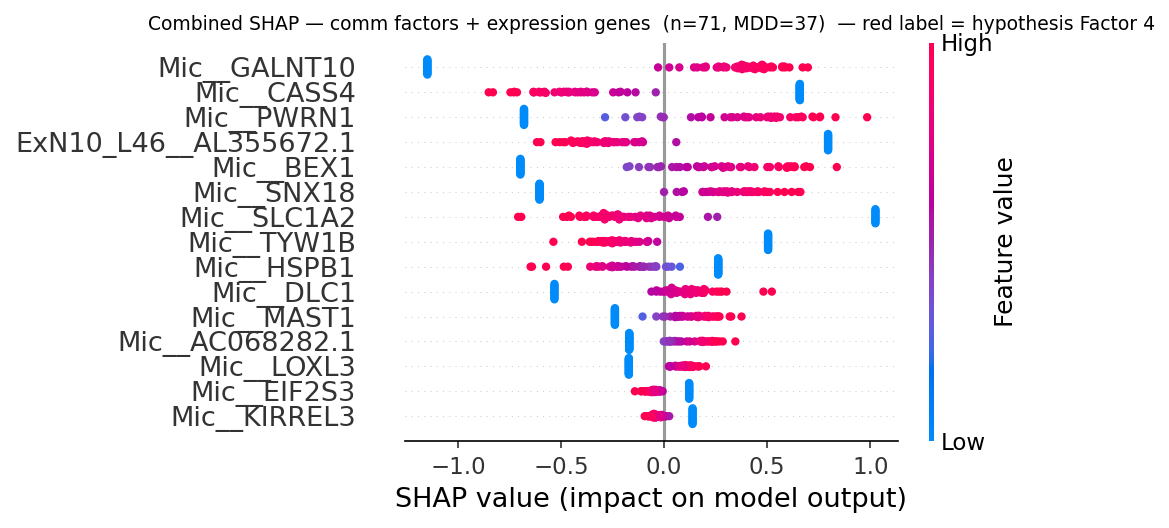
\includegraphics[width=\linewidth]{figures/step4_shap_beeswarm_combined_overall.png}
  \caption{Combined space: factors vs.\ genes. mRMR keeps 15 genes (mostly
  \code{Mic\_\_*}); all 5 factors are dropped.}
  \label{fig:beeswarm-combined}
\end{subfigure}\hfill
\begin{subfigure}{0.49\textwidth}
  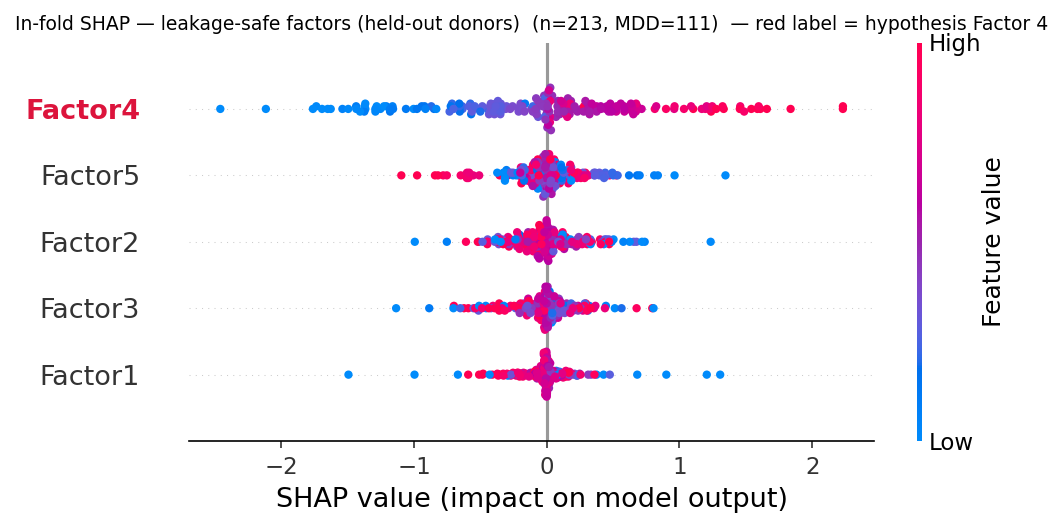
\includegraphics[width=\linewidth]{figures/step4_shap_beeswarm_infold_overall.png}
  \caption{In-fold leakage-safe factors on held-out donors, pooled across the
  3 CV rounds ($71\times3=213$ held-out predictions): \factorfour\ becomes the
  \#1 communication factor.}
  \label{fig:beeswarm-infold}
\end{subfigure}
\caption{The two extended SHAP views. Left: when factors and genes compete, the
genes win and \factorfour\ is redundant for prediction. Right: among
communication features alone (leakage-safe), \factorfour\ dominates.}
\label{fig:beeswarm-ext}
\end{figure}

% ===========================================================================
\section{Discussion}
% ===========================================================================

The results form a coherent, non-contradictory picture. The
microglia\,$\rightarrow$\,\code{ExN10\_L46} communication program (\factorfour)
is the \emph{dominant, reproducible} communication signal in this dataset: it
self-separates from the strong cohort/batch confound (which collapses into
Factors~2/3/5), it leans toward MDD in both sexes, and it becomes the single
most important communication feature once factors are re-estimated leakage-free.
This \textbf{directionally supports} the central hypothesis that a shared
microglia\,$\rightarrow$\,neuron axis---not two unrelated sex-specific
findings---underlies the female-microglial and male-neuronal signals reported by
Maitra \textit{et al.} The L--R drivers (synaptic-adhesion, glutamatergic and
Ca$^{2+}$ signalling, including the psychiatric-risk genes \code{CACNA1C} and
\code{IL1RAPL1}) are biologically sensible for a microglia--neuron synaptic
interface.

\textbf{But the communication \emph{representation} adds no predictive value
over expression.} When factors and genes compete, mRMR discards every factor in
favour of microglial genes, and the combined classifier never CI-separates from
the expression baseline. This is expected rather than paradoxical:
communication is \emph{derived from} expression, and a rank-5 program is a
compressed, lossy summary of the same microglial transcriptional state that the
raw \code{Mic\_\_*} genes encode at full resolution. At $n=71$ the compression
buys interpretability, not discriminative power. The signal is \emph{real but
not independent}. Note the comparison is, if anything, \emph{conservative}: the
expression baseline already includes per-cell-type pseudobulk for
\code{ExN10\_L46}---the very receiver of the hypothesis axis---so the factors
compete against a baseline deliberately favourable to the hypothesis and still
add nothing.

% ===========================================================================
\subsection{Limitations}
% ===========================================================================

\begin{itemize}
\item \textbf{Sample size.} $n=71$ donors with $\sim$50/50 labels gives wide
bootstrap CIs; a $+0.05$~AUC value-add is not resolvable. This is the binding
constraint and the reason no GNN was attempted.
\item \textbf{Sex\,$=$\,cohort confound.} Females and males come from separate
libraries, so cross-sex generalisation cannot be cleanly tested; we use within-sex
pooled CV instead, which tests value-add but not transfer.
\item \textbf{\factorfour\ is not pure microglia.} Its top sender is Endothelial
(0.79) above Microglia (0.40); it is best described as a non-neuronal
(vascular\,+\,immune)\,$\rightarrow$\,deep-layer-neuron program. The directed
test is justified by a priori biological selection, not by the $p$-value.
\item \textbf{Trend-level univariate signal.} \factorfour's diagnosis
association is $p=0.057$ (a trend), and the male standalone $p=0.05$ is
borderline.
\item \textbf{Microglia recovery is sex/cohort-skewed} (female 46 vs.\ male 16
median nuclei/donor), a batch effect reinforced by Factors~2/3/5.
\item \textbf{Pseudoreplication} affects the nucleus-level DEG sanity check;
donor-level pseudobulk is the fix used everywhere downstream.
\end{itemize}

% ===========================================================================
\section{Conclusion}
% ===========================================================================

Modelling cell--cell communication explicitly recovers a single, reproducible
microglia\,$\rightarrow$\,\code{ExN10\_L46} program that is elevated in MDD
donors of both sexes and is the most important communication feature under
leakage-safe estimation---\emph{directionally supporting} the hypothesis that the
female-microglial and male-neuronal MDD signals are two ends of one axis. The
biology is supported. However, this communication representation carries
\emph{no predictive information independent of microglial gene expression} at
$n=71$: when the two compete, expression wins and the factors are dropped. The
honest conclusion for a course project is therefore a \emph{qualified yes}---the
shared axis is visible and real, but it is a low-rank shadow of microglial
transcriptional state rather than an independent, value-adding signal.

% ===========================================================================
\section*{Data and code availability}
% ===========================================================================

\paragraph{Data.} All data are public. The dlPFC snRNA-seq count matrices and
metadata were obtained from the Gene Expression Omnibus under accessions
\textbf{GSE213982} (female cohort; the released combined counts matrix also
contains the male nuclei) and \textbf{GSE144136} (male cohort metadata),
published by Maitra \textit{et al.}~\cite{maitra2023}. No new data were
generated by this project.

\paragraph{Code.} All analysis code is openly available at\\
\url{https://gitlab.com/boulgeo/MLCB_team_project}\\
(mirrored at \url{https://github.com/GiorgosBoulogeorgos/MLCB_team_project}),
organised as \code{src/} (library modules), \code{notebooks/} (phase-by-phase
runners) and \code{report/} (this manuscript and its figures). Key modules:
\code{src/functions.py} (Phases~A/B), \code{src/pseudobulk.py} (donor-level
pseudobulk), \code{src/tensor\_features.py} (in-fold tensor projector),
\code{src/rncv.py} (repeated nested cross-validation),
\code{src/feature\_selection.py} (\code{VarianceTopK}, \code{MRMRSelector}),
\code{src/estimators.py} (the five classifiers and their Optuna search spaces)
and \code{src/shap\_step4.py} (Phase~D interpretability); the end-to-end
rigorous run is reproduced by \code{run\_rigorous\_local.py}. Raw data and
intermediate checkpoints are not committed (they exceed repository limits) and
are regenerated from GEO by the Phase~A notebook.

\paragraph{Reproducibility settings.} Rigorous run: seed~42,
3$\times$5$\times$3 repeated nested CV, 20 Optuna trials per inner search,
per-fold tensor refit; LIANA~1.7.3 / cell2cell~0.8.4 for Phase~B. Each expensive
step is checkpointed, so a runtime timeout never costs more than one step.

% ===========================================================================
\section*{Author contributions}
% ===========================================================================

\textbf{G.B.} conceived the study: he wrote the original project proposal,
formulated the microglia\,$\rightarrow$\,neuron shared-axis hypothesis and
designed the proposed pipeline, which was then discussed and refined jointly
with A.M. \textbf{A.M.} carried out Phase~A (data loading, annotation, QC and
the reproduction of the cell-type signal). \textbf{G.B.} carried out Phase~B
(per-donor LIANA inference, tensor construction and the non-negative CP
decomposition) and Phase~C (pseudobulk feature construction, the three feature
sets, the leakage-controlled repeated nested cross-validation and the
in-fold tensor projector), and contributed to Phase~D. \textbf{A.M.} completed
Phase~D (SHAP-based interpretation of the models and of \factorfour, and the
directed hypothesis test), led the interpretation of the results and prepared
the presentation slides. \textbf{Both authors} wrote the manuscript jointly,
discussed the methodology throughout, reviewed the analyses, and read and
approved the final version.

% ===========================================================================
\section*{AI usage disclosure}
% ===========================================================================

In line with good scientific practice, we disclose that generative AI
(\textbf{Anthropic's Claude}) was used as a coding and writing assistant during
this project. Specifically, it was used to (i)~produce the \emph{initial
scaffold} of the analysis pipeline (module and notebook skeletons, function
signatures, boilerplate); (ii)~\emph{debug code}, most substantially in the
Phase~B LIANA / tensor-decomposition stage (e.g.\ diagnosing the missing
$-\log_{10}$ transform of the \code{magnitude\_rank} score, which had inverted
the in-fold factors); (iii)~\emph{generate figures} (the plotting code for the
SHAP beeswarms, the reconstruction-error curve and the pipeline diagram); and
(iv)~perform \emph{code review} of the analysis modules.

No AI system was used to generate data, to fabricate or alter results, or to
decide the scientific conclusions. The study design, hypothesis, methodological
choices, evaluation protocol, interpretation of the results and the claims made
in this manuscript are the authors' own. All AI-assisted code was read, tested
and validated by the authors, and all AI-assisted text was reviewed and edited
by them. The authors take full responsibility for the entire content of this
work.

% ===========================================================================
\section*{Competing interests}
% ===========================================================================

The authors declare no competing interests.

% ===========================================================================
\begin{thebibliography}{99}

\bibitem{maitra2023}
M.~Maitra \textit{et al.},
``Cell type specific transcriptomic differences in depression show similar
patterns between males and females but implicate distinct cell types and genes,''
\textit{Nature Communications} \textbf{14}, 2912 (2023).
GEO: GSE213982, GSE144136.

\bibitem{liana2022}
D.~Dimitrov \textit{et al.},
``Comparison of methods and resources for cell-cell communication inference from
single-cell RNA-Seq data,''
\textit{Nature Communications} \textbf{13}, 3224 (2022). (LIANA.)

\bibitem{tensorc2c}
E.~Armingol \textit{et al.},
``Context-aware deconvolution of cell--cell communication with
Tensor-cell2cell,''
\textit{Nature Communications} \textbf{13}, 3665 (2022).

\bibitem{tensorly}
J.~Kossaifi, Y.~Panagakis, A.~Anandkumar, M.~Pantic,
``TensorLy: Tensor learning in Python,''
\textit{Journal of Machine Learning Research} \textbf{20}(26), 1--6 (2019).

\bibitem{shap}
S.~M.~Lundberg and S.-I.~Lee,
``A unified approach to interpreting model predictions,''
\textit{Advances in Neural Information Processing Systems (NeurIPS)} \textbf{30}
(2017). (SHAP.)

\bibitem{xgboost}
T.~Chen and C.~Guestrin,
``XGBoost: A scalable tree boosting system,''
\textit{Proc.\ 22nd ACM SIGKDD}, 785--794 (2016).

\bibitem{mrmr}
H.~Peng, F.~Long, and C.~Ding,
``Feature selection based on mutual information: criteria of max-dependency,
max-relevance, and min-redundancy,''
\textit{IEEE Trans.\ Pattern Analysis and Machine Intelligence} \textbf{27}(8),
1226--1238 (2005). (mRMR.)

\bibitem{scanpy}
F.~A.~Wolf, P.~Angerer, F.~J.~Theis,
``SCANPY: large-scale single-cell gene expression data analysis,''
\textit{Genome Biology} \textbf{19}, 15 (2018).

\bibitem{sklearn}
F.~Pedregosa \textit{et al.},
``Scikit-learn: Machine learning in Python,''
\textit{Journal of Machine Learning Research} \textbf{12}, 2825--2830 (2011).

\bibitem{optuna}
T.~Akiba, S.~Sano, T.~Yanase, T.~Ohta, M.~Koyama,
``Optuna: A next-generation hyperparameter optimization framework,''
\textit{Proc.\ 25th ACM SIGKDD}, 2623--2631 (2019).

\end{thebibliography}

\end{document}
